\documentclass[a4paper,10pt]{article}
\usepackage[utf8x]{inputenc}
\usepackage{algorithmic}
\usepackage{algorithm}
\usepackage{graphicx}

\usepackage{common-formatting}
\usepackage{common-math}

%opening
\title{TP1 - Projets déterministes - MACS1}
\author{Alexandru Fikl}

\begin{document}

\maketitle

\section{Décomposition LU}
\begin{prop}
    Soit $A \in \field{K}^{n, n}$ telle que toutes ces sous-matrices soient inversibles,
alors il existe un unique couple $(L, U)$ tel que $A = LU$, avec L matrice triangulaire
inférieur avec diagonale unité et U matrice triangulaire supérieure.
\end{prop}
\vspace*{-15pt}
\[
\overbrace{
 \begin{pmatrix}
  a_{1,1} & a_{1,2} & \cdots & a_{1,n} \\
  a_{2,1} & a_{2,2} & \cdots & a_{2,n} \\
  \vdots  & \vdots  & \ddots & \vdots  \\
  a_{n,1} & a_{n,2} & \cdots & a_{n,n}
 \end{pmatrix}}^{\displaystyle A}
 =
 \overbrace{
 \begin{pmatrix}
  1 & 0 & \cdots & 0 \\
  l_{2,1} & 1 & \cdots & 0 \\
  \vdots  & \vdots  & \ddots & \vdots  \\
  l_{n,1} & l_{n,2} & \cdots & 1
 \end{pmatrix}}^{\displaystyle L}
 \overbrace{
 \begin{pmatrix}
  u_{1,1} & u_{1,2} & \cdots & u_{1,n} \\
  0 & u_{2,2} & \cdots & u_{2,n} \\
  \vdots  & \vdots  & \ddots & \vdots  \\
  0 & 0 & \cdots & u_{n,n}
 \end{pmatrix}}^{\displaystyle U}
\]

\textbf{Calcul explicite de la décomposition LU}:
\begin{enumerate}
    \item Ecrire ce que vaut $a_{i, j}$ coefficient $(i, j)$ de $A = LU$.
\[
a_{i, j} = \sum_{k = 0}^n l_{i, k} u_{k, j}.
\]

    \item Que vaut $l_{i, k}$ lorsque $k \geq i + 1$? Que vaut $u_{k, j}$ lorsque
$k \geq j + 1$? Reécrire la somme $a_{i, j}$ en conséquence.

\begin{align*}
l_{i, k}& = 0,\text{ pour } k \geq i + 1. \\
u_{k, j}& = 0,\text{ pour } k \geq j + 1. \\
a_{i, j}& = \sum_{k = 0}^i l_{i, k} u_{k, j}.
\end{align*}

    \item Calcul sur la première colonne: que vaut $a_{i, 1}$? En déduire $l_{i, 1}$.
\[
    a_{i, 1} = l_{i, 1} u_{1, 1} \implies l_{i, 1} = \frac{a_{i, 1}}{u{1, 1}}.
\]

    \item Calcul sur les colonnes j ($2 \leq j \leq n$): on suppose ccoonnues les colonnes
    de L et U pour $k$ allant de 1 à $j - 1$. Ecreire ce que vaut $a_{i, j}$ pour
    $1 \leq i \leq j$ puis pour $j + 1 \leq u \leq n$. En déduire $u_{i, j}$ pour
    $1 \leq i \leq j$ et aussi $l_{i, j}$ pour $j + 1 \leq i \leq n$.
\begin{align*}
a_{i, j}& = \sum_{k = 0}^i l_{i, k} u_{k, j}, \text{ pour } 1 \leq i \leq j. \\
a_{i, j}& = \sum_{k = 0}^j l_{i, k} u_{k, j}, \text{ pour } j + 1 \leq i \leq n. \\
u_{i, j}& = a_{i, j} - \sum_{k = 0}^{i - 1} l_{i, k} u_{k, j}. \\
l_{i, j}& = \displaystyle \frac{a_{i, j} - \sum_{k = 0}^{i - 1} l_{i, k} u_{k, j}}{u_{j, j}}.
\end{align*}

    \item Ecrire le pseudo-code de l'algorithme de décomposition LU.
\begin{algorithm}
\caption{Décomposition LU}
\begin{algorithmic}
\STATE $A \in \mathcal{M}_{n, n}(\field{K})$
\STATE $L = I_n$
\STATE $U = O_n$
\FOR{$i := 1 \to n$}
    \FOR{$j := i \to n$}
        \STATE $u_{i, j} = a_{i, j} - \sum_{k = 1}^n l_{i, k}u_{k, j}$
    \ENDFOR

    \FOR{$j := i + 1 \to n$}
        \STATE $l_{j, i} = \displaystyle \frac{a_{i, j} - \sum_{k = 1}^{i - 1} l_{i, k} u_{k, j}}{u_{j, j}}$
    \ENDFOR
\ENDFOR
\end{algorithmic}
\end{algorithm}

    \item (voir le ficher \emph{LUDecomposition.m}).
    \item (voir les fichers \emph{ResolveLower.m} et \emph{ResolveUpper.m}).
    \item (voir les fichers \emph{main\_lu.m} et \emph{solveSystem.m}).
    \item (voir le ficher \emph{main\_lu.m}).
\end{enumerate}

\section{Moindres carrés}
\begin{prop}
    Soit $A \in \field{R}^{n, p}$ et $b \in \field{R}^n$. Le problème de moindres carrés $\norm{Ax - b}
= \min_{y \in \field{R}^p} \norm{Ay - b}{}$ admet au moins une solution. De plus cette
solution est unique si et seulement si $\ker(A) = \emptyset$.
\end{prop}

\begin{prop}
$x \in \field{R}^p$ est solution du problème de moindre carré précédent si et seulement si
x est solution de $A^T A x = A^T b$.
\end{prop}

\begin{enumerate}
    \item Construire une matrice $A$ de taille $n > p$ tel que $Ker(A) = \emptyset$.
Construire un vecteur $b$ de taille $n$ tel que $b \notin Im(A)$. Donner des examples
pour $p = 2$ et $p = 3$.

\hbox{}

Soient:
\[
A_1 =
\begin{pmatrix}
  7 & 1 \\
  5 & 5 \\
  4 & 3 \\
  1 & 9
\end{pmatrix}
\text{ et } b_1 =
\begin{pmatrix}
  1 \\
  0 \\
  0 \\
  0
\end{pmatrix}
\]

\[
A_2 =
\begin{pmatrix}
  2 & 7 & 1 \\
  3 & 5 & 5 \\
  9 & 4 & 3 \\
  6 & 1 & 9 \\
  8 & 3 & 1
\end{pmatrix}
\text{ et } b_2 =
\begin{pmatrix}
  1 \\
  0 \\
  0 \\
  0 \\
  0
\end{pmatrix}
\]

Le rang des matrices $A_1$ et $A_2$ est 2, respectivement 3, donc leur noyau est nul.
Aussi, les vecteurs $b_1$ et $b_2$ ne sont pas dans $Im(A_1)$, respectivement $Im(A_2)$.
Les solutions aux equations $A_1^TA_1x_1 = A_1^Tb_1$ et $A_2^TA_2x_2 = A_2^Tb_2$ sont:
\[
x_1 =
\begin{pmatrix}
  0.0979 \\
  -0.0361
\end{pmatrix}
\text{ et } x_2 =
\begin{pmatrix}
  -0.0400 \\
  0.1132 \\
  -0.0094
\end{pmatrix}
\]
    \item (voir les fichers \emph{main\_leastsquares.m} et \emph{testLeastSquares.m}).
\end{enumerate}

\begin{figure}[h]
    \centering
    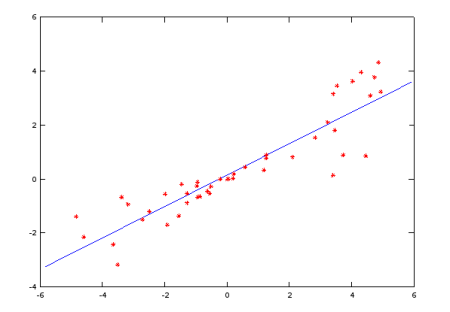
\includegraphics{./img/line.png}
    \caption{Approximation par une droite}
\end{figure}

\begin{figure}
    \centering
    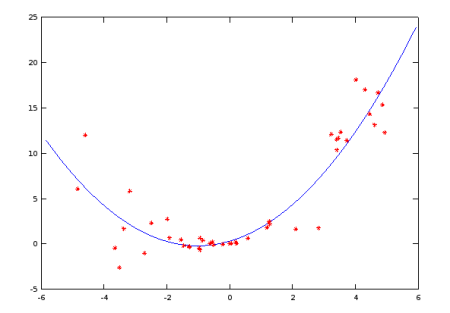
\includegraphics{./img/parabola.png}
    \caption{Approximation par une parabole}
\end{figure}

\begin{figure}
    \centering
    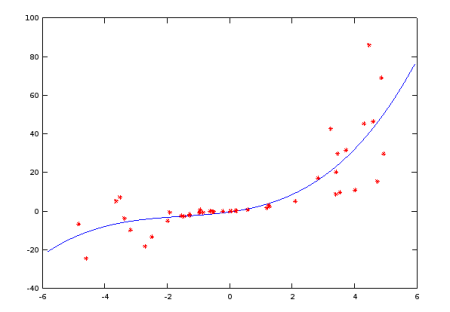
\includegraphics{./img/spline.png}
    \caption{Approximation par une courbe cubique}
\end{figure}

\end{document}
